\chapter{Theory}
\label{chapter:theory}

Here, the theory behind our methods are further described. In order to give an overview of the context of the research, a general description of ambiguities in languages, grammars and probabilistic language models is given. Grammatical Framework, Universal Dependencies and Wordnet are three important resources for the methods in this thesis and are also described. Last, we give an account of the theoretical foundations of the Expectation Maximization algorithm.


\section{Ambiguities in Language}
\label{section:ambiguities}

% \begin{itemize}
%     \item What is a ambiguity in general
%     \item Structural ambiguities
%     \item ``I eat the food in the kitchen''
%     \item Lexical ambiguities
% \end{itemize}
% \vspace{5mm}

When interpreting a sentence, ambiguities in natural language will inevitably be a problem.  We will here introduce two kind of natural language ambiguities: lexical ambiguity and syntactic ambiguity. 

A simple example of a lexical ambiguity in natural language is the word ``bass''. It might refer to a type of fish in one sentence (I am fishing bass) and to a type of instrument in another (I play the bass). These kind of ambiguities is highly language dependent and words are often ambiguous in different ways in different languages. As an example the Swedish words for bass the fish and bass the instrument are different (aborre vs. bas).

To understand syntactic ambiguity, we look at the sentence ``I eat the food in the kitchen'', where the clause ``in the kitchen'' could potentially refer either to the location where the eating is done or as an attribute to the food that was eaten (``I am in the kitchen and I eat the food'' or ``I eat the food that is in the kitchen''). This kind of ambiguity does not depend on the vocabulary of the language, but on the grammar. Depending on the intended meaning, this sentence would be translated differently into Chinese as we can see in the following example:

% Enable Chinese input
\begin{CJK*}{UTF8}{gbsn}
\begin{exe}
\label{eat_food_example}
\ex 
\glll 我 在 厨房 吃 饭\\
wo zai chufang chi fan\\
I in kitchen eat food.\\
\trans `I eat the food in the kitchen'
\ex 
\glll 我 吃 在 厨房 的 饭\\
wo chi zai chufang de fan\\
I eat in kitchen [attributive] food\\
\trans `I eat the food in the kitchen'
\end{exe}
\end{CJK*}

These two examples illustrates that there are sentences that are syntactically ambiguous in one language but not in others. This has great implications for applications such as machine translation, as there must be a model describing how to choose the right interpretation of a sentence in order to make the correct translation. \todo{Need citation}

%suggest that it is possible to make use of information from other languages when disambiguating different interpretation of a sentence.


\section{Grammars and Syntax}
% \begin{itemize}
% \item Natural language can be analyzed syntactically using tree structures. 
% \item Information about what a grammar is
% \begin{itemize}
%     \item Constituency grammars
%     \item Dependency grammars
% \end{itemize}
% \item Constituency grammars have production rules that iteratively converts symbols to a set of terminal symbols (words)
% \item Can be visualized with a syntax tree

% \item Constituency compared to dependency grammar (see figure \ref{fig:depconst})
% \begin{itemize}
% \item The difference between constituency grammar and dependency grammars
% \item Constituency trees contain more information
% \item Constituency trees show how a group of words acts as one unit
% \item Dependency grammars describe relations between words and defines a tree over the words themselves  \citep{nivre2005dependency}
% \end{itemize}
% \end{itemize}
% \vspace{5mm}

In linguistics, \textbf{syntax} is a set of formal rules that governs how sentences are constructed and structured in a given language, such as in which order the subject, the verb and the object should appear \citep{chomsky2002syntactic}. Together with the \textbf{morphology}, how individual words change in a language depending on the sentence they are in, these rules constitute the \textbf{grammar} of the language. 

One type of grammars are phrase structure grammars, which focus on describing a sentence by identifying sub-phrases in the sentence recursively. A simple example of this is how in the sentence \emph{Bob kicks the green ball} one can identify \emph{kicks the green ball} as functioning as a verbal phrase in which one in turn can identify \emph{the green ball} to function as a noun phrase. A different type of grammar is called \textbf{dependency grammar}. The focus of this type of grammar is on the relationship between words \citep{nivre2005dependency}, for example, in the same sentence, one can identify the words \emph{Bob} and \emph{ball} as depending on \emph{kicks} and \emph{green} as depending on \emph{ball}. In both these cases the rules of the grammar can be used to draw up a hierarchical tree, called a syntax tree, that describes which rules were used to build a certain sentence. Examples of phrase structure trees and dependency trees are displayed in figure \ref{fig:depconst}. %There are examples of grammars where one can extract the dependency tree from a phrase structure tree using rule-based transformations; this is how the Stanford parser parses text into dependency trees \citep{de2006generating}.

The process of deciding the syntax tree of a given sentence is called \textbf{parsing}. This process is non-trivial because in many cases it is non-deterministic, for one given sentence there can be many different valid syntax trees. An example is the sentence \emph{I eat the food in the kitchen} treated in section \ref{section:ambiguities} which as can be seen in figure \ref{fig:depconst} have different syntax trees depending on the interpretation of the sentence. The fact that syntax trees can serve to formalize which of the many syntactic interpretations a sentence could have makes it an excellent tool for use in computers understanding and processing language and there are many machine translation systems that use syntactic analysis as a key method.
%\todo{citation needed}


%%% TODO
%Syntax trees disambiguate syntactic ambiguity
% WORDNET - disambiguates lexical ambiguity
% GF/ABSTRACT SYNTAX - Extract those parts of syntax that disambiguate syntactic ambiguity but abstract away descriptions of "tradidional syntax" "how the language is read and written", also takes into account 



\begin{figure}
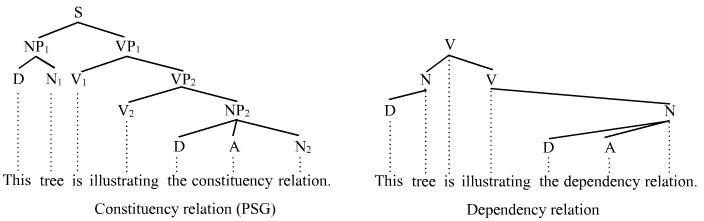
\includegraphics[width=\linewidth]{figure/dependency_constituency.png} 
\caption{Trees illustrating the dependency and constituency relations, adapted from \citet{wikipedia2011trees}.}
\label{fig:depconst}
\end{figure}

\section{Probabilistic Language Models}
\label{sec:lm}

Probabilistic models for language work by computing the probability of observing a certain type of linguistic item in text or speech. Examples of such models are language models that assign probabilities to sentences or fragments of sentences in a certain language, such as n-gram models. One can also define probabilistic models over possible interpretations of the same sentence, such as the different valid syntax trees of a sentence which can then be used as a toll for disambiguation tasks.

\subsection{N-gram models}
N-gram models are generative models in the sense that they assume that the probability of a certain word appearing in a sentence only depends on the history of that word, that is the words preceding it, and that the probability of a word occurring is location invariant. More specifically, n-gram models assumes that the probability of a certain word appearing only depends on the previous $n$ words for some fixed $n$ \citep{jurafsky2009speech}. These models can assign a certain probability to every possible sentence by using the chain rule, can be used to predict the next word in a sentence, and can easily be used generatively to sample new sentences according to the probability distribution defined by the model. N-gram models are well researched and are considered one of the most important tools in speech and language processing.\todo{Citation?}

\citet{jurafsky2009speech} writes that for most disambiguation tasks for natural language probabilistic or statistical models are used. As opposed to general language models, such as n-gram models, the types of probabilistic models used for disambiguation work by instead of assigning a probability to each sentence computing the probability that a certain sentence should be interpreted in a certain way in face of ambiguity. A model for syntactic disambiguation could for example define a probabilistic model assigning probabilities for all possible syntax trees of a sentence. With such a model disambiguation can then be done by computing the probability for each possible interpretation and choosing the one with the highest probability.

\subsection{Probabilistic context free grammars}
Among probabilistic grammar models for phrase structure grammars the most common ones are \textbf{Probabilistic Context Free Grammars} (PCFG). According to \citet{manning1999foundations}, PCFG:s adhere to the three assumptions of place invariance, context freeness, and ancestor freeness. Place invariance means that the probability of a sub-tree of the syntax tree occurring does not depend on where in the sentence the words that subtree spans are. As such a certain noun phrase would have the same probability irregardless of whether it is first or last in the sentence. Context freeness means that the probability of a given subtree does not depend on any words outside the span of that sub-tree. For example, the probability of a given noun phrase does not depend on the main verb in the sentence. Lastly ancestor freeness means that the probability of a subtree does not depend on any nodes outside that subtree, for example the probability of a given noun phrase would not depend on it being a part of a verb phrase or a prepositional phrase.

It is obvious that these assumptions does not hold for real text and \citet{jurafsky2009speech} indeed writes that the main drawback of the PCFG is that the sweeping independence assumptions automatically discards many structural dependencies in the syntax tree. In addition it is also insensitive to lexical information. This can be somewhat remedied by various modifications to the PCFG and \citet{jurafsky2009speech} mentions techniques such as \textbf{lexicalization} and \textbf{splitting non terminals}. 

\subsection{Syntactic n-grams over dependency trees}
In order to improve the n-gram model \citet{sidorov2014syntactic} introduced \textbf{syntactic n-grams}. These differs from ordinary n-grams in what is considered the history in the model. Instead of defining the history as the previous words in the original sentence order, a syntactic n-gram instead considers the predecessors in a \textbf{dependency tree} of the sentence as the history of a word. This allows for some long range dependencies to be accounted for easier than in a normal linear n-gram model. For example, in \emph{bob kicks the green ball} the word \emph{kicks} is the immediate predecessor of \emph{ball} in the dependency tree and the predictive information of \emph{kicking ball} occurring often together would be captured using only a syntactic bigram model, in the linear n-gram case, this particular case would require a 5-gram model in order to be able to capture the same relation. Due to the fact that word order is a highly language dependent property, syntactic n-grams are more suited for cross-lingual comparison \citep{sidorov2014syntactic}.% which is a vital property for our work. %In our work we will consider syntactic bigrams, which, even given the limited size, was showed by \citet{sidorov2014syntactic} to contain linguistic information that ordinary n-grams was not able to capture.

A more generalized generative language model based on the syntactic nature of the dependency tree structure is developed by \citet{richardson2016generalized}. \citeauthor{richardson2016generalized} defines the history of each node in the tree as all nodes preceding that node given a defined traversal order. By denoting the $i$:th node in the tree $w_i$ and the history of the $i$:th node (that is all nodes preceding $w_i$) as $H_i$, \citeauthor{richardson2016generalized}  also defines the `$t$-treelets of size $l$ for $w_i$' as all connected subtrees $S'\subset H_i$ where $w_i\in S'$ and $|S|=l$. $t$-treelets can be divided into several types depending on the topology of the trees and a generative probabilistic model can be defined by assuming that the probability of a certain node given its history is equal to the probability of a node given all $t$-treelets for the node that are of certain type and size. Examples of such models are all $t$-treelets of size $l\leq 3$ that only consists of nodes that are ancestors to $w_i$ or all $t$-treelets of size $l=3$ that only consists of the parent node and one sibling node to $w_i$. The fact that one needs a well defined traversal order of the tree to define the history of each node is important in order to create a generative model, as there would otherwise appear circular dependencies in the model. 

\todo{Do we want a more theoretical/mathematical explanation of how to define tree probabilities like we do in method chapter? Maybe try to find references for that method and present it as theory instead}

% \begin{itemize}
%     \item Statistical syntactic models
%     \item Used for disambiguation
%     \item Interpretation depends on context, local vs long range content
%     \item The assumptions of probabilistic context free parsing \citep{manning1999foundations}
%     \item Context freeness
%     \item Ancestor freeness
%     \item Place invariance
%     \item We want to break context invariance
%     \item Example of contextual information
%     \begin{itemize}
%         \item Pronouns is more common as a subject than as an object to a verb
%     \end{itemize}
%     \item Lexicalization \citep{jurafsky2009speech}
% \end{itemize}

\section{GF and Abstract Grammars}
% \begin{itemize}
%     \item Background GF
%     \item GF is a formalism for multilingual grammars \citep{ranta2004computational}
%     \item Originally focused on controlled natural language, now also extanded
%     \item The problem: grammars are defined for one language only, there is no way to ``convert'' them or reuse resources across languages
%     \item The assumption: Languages share an underlying structure that manifests in different ways for different languages
%     \item The solution: Divide the grammar into abstract and concrete parts
%     \item What does abstract mean in this sense?
%     \item Types of grammars in GF (PMCFG)
% \end{itemize}
Grammatical Framework \citep{ranta2004grammatical} is a framework for writing and implementing formal grammars grammars in particular for natural languages. The defining feature is that grammars are divided into an \textbf{abstract syntax} and a \textbf{concrete syntax}, a concept borrowed from programming language design. According to \citeauthor{ranta2004grammatical} the abstract syntax defines ``the hierarchical structure of the language'' and the concrete syntax ``what the language looks like as it is read and written''. In GF different languages can share the same abstract syntax describing the semantics, i.e. the meaning, of statements in \emph{all} languages, while each language has its distinct concrete syntax. The concrete syntax can be seen as a description of how the abstract syntax should be rendered in the textual form of the corresponding language, which means that by describing a statement in abstract syntax we can \textbf{linearize} that statement to the textual versions of that statement into all supported languages. \citet{angelov2009incremental} then describes a method to \textbf{parse} text to get all valid representations in abstract syntax for a statement given in linearized textual form in a language that have a defined concrete grammar over the abstract syntax.

Together, the ability to parse and linearize statements for all languages with a concrete syntax over the same abstract syntax means that meaning preserving translation is possible between those languages, in effect using the abstract syntax as a \textbf{pivot language} or an \textbf{interlingua}. In figure \ref{fig:abstract_translation} \todo{fix figure} an illustration of how this approach works can be seen. The main problem in doing translation by this approach is that the parsing step in many cases is not deterministic, that is for a given statement in textual form there might be several valid abstract representations of that statement. This is not surprising in and is in fact unavoidable if one wants the abstract syntax to accurately describe the semantic meaning of each statement, and for accurate translation using the interlingua approach to work. As an example, the ambiguous sentences given in section \ref{section:ambiguities}, ``I like bass'' and ``I eat the food in the kitchen'' would have different abstract representations depending on the interpretation of each sentence, and must be \textbf{disambiguated} in order to be translated accurately to Swedish and Chinese respectively. That means that one must choose which of the possible abstract representations should be used as the immediate representation. 

The algorithm for fast statistical parsing presented by \citet{angelov2014fast} introduces a statistical element to parsing by giving each possible abstract parse a probability score that aims to reflect the likelihood of a given possible abstract representation being the correct one. \citeauthor{angelov2014fast}'s parsing method has many similarities to the PCFG method and can indeed be seen as being a context free probabilistic model in the abstract domain.\todo{citation needed} \citet{virk2014developing} also use statistical parsing of abstract syntax trees together with word sense disambiguation to disambiguate lexical ambiguities to show that it is possible to parse arbitrary English text, and show improvements in translation with the interlingua approach using GF.
%The type of grammars used in Grammatical Frameworks are a type of \emph{parallel multiple context free grammars} (PMCFG) and are mainly used to describe and formalize the structure of sentences in natural languages. The grammars consist of two parts, the abstract and the concrete part. The abstract part can be seen as a more general form and can be shared between several languages, while the concrete part contains all language specific rules of a language such as vocabulary, morphology and word order and is basically a way to transform the abstract syntax into the corresponding sentence in the language.

%The abstract part of a grammar can be seen as an interlingua called abstract syntax and consists of a set of \emph{symbols} and a set of \emph{production rules}, each rule transforming one symbol to one or several other symbols. These rules can be applied recursively to ultimately produce a set of \emph{terminal symbols}, symbols which can't be further transformed by any production rule. The abstract syntax describes through what symbols and production rules a set of terminal symbols were produced. The production rules can be seen as a set of universal grammatical rules, for example that a verb phrase could consist of one transitive verb and a noun. The rules and symbols used to obtain a certain set of terminal symbols can be described with a tree structure, and are thus called an \emph{abstract syntax tree}. This tree has an initial symbol as its root node, the intermediate symbols obtained when applying rules as its intermediate nodes and the terminal symbols as its leaf-nodes. 

%An example of an abstract syntax tree can be seen in figure X. The chain of production rules this AST represents is one rule transforming the initial symbol \emph{clause} to the intermediate symbols \emph{noun} and \emph{verb phrase}, then another transforming the \emph{verb phrase} to one \emph{transitive verb} and one \emph{noun}, the two \emph{noun}:s and the \emph{transitive verb} might then each be transformed to terminal symbols carrying the meaning of ``horse'', ``eat'' and ``hay'' respectively. Note that the first noun was actually transformed to two symbols, where one of the symbols indicate that the noun is expressed in the plural number. This path of production and the associated syntax tree, carries the meaning of the English sentence ``horses eat hay'' and would indeed produce that sentence when linearizing the abstract syntax using the concrete rules of a properly defined English concrete model. However this abstract syntax tree is not specific for the English grammar, but given a proper Swedish concrete grammar for the same abstract grammar this AST could also linearize to the same sentence in Swedish (which would be ``hästar äter hö'').

%In Grammatical Framework, the problem of disambiguating abstract syntax trees includes both lexical disambiguation and syntactic disambiguation in that the word sense information for each word of a sentence must be present in the correct abstract syntax tree of the sentence in order for it to be a truly language independent representation of the meaning of the sentence.

\begin{figure}[!htbp]
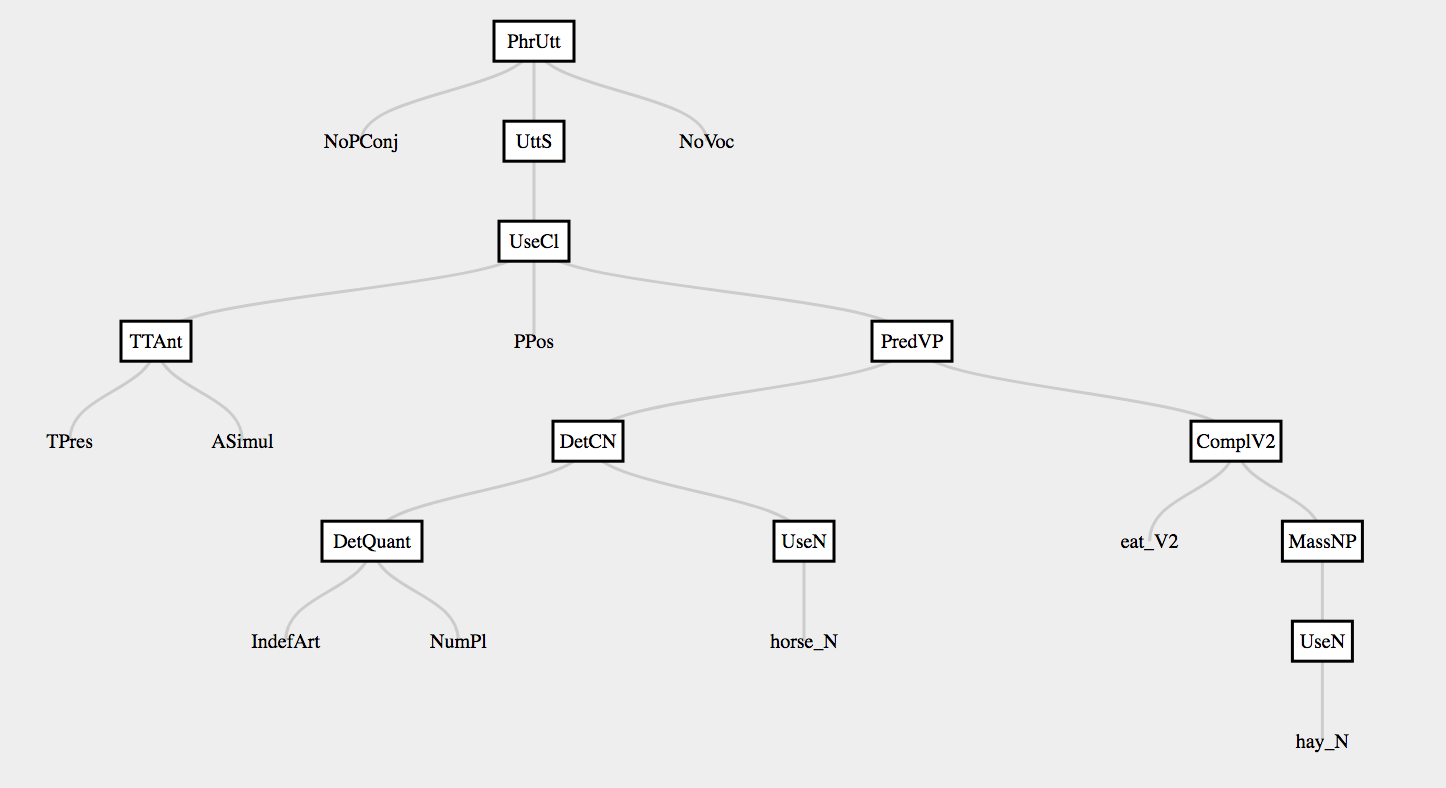
\includegraphics[width=\linewidth]{figure/ast}
\caption{Example of an abstract syntax three from the GF runtime representing the English sentence ``Horses eat hay''.}
\label{fig:ast}
\end{figure}

\section{Universal Dependencies}
%\begin{itemize}
%    \item Language independent dependency grammar annotation scheme
%    \item Fixed set of dependency labels and part of speech tags
%    \item Wide array of treebanks for different languages
%    \item There is work on a mapping gf2ud and ud2gf
%    \item The gf/ud relationship is one to many, and the UD standard does not encompass the notion of abstract functions so these is not inherent WSD
%    \item Introduce the concept of abstract dependency tree from GF2UD paper
%\end{itemize}
%\vspace{5mm}
Universal dependencies is an annotation scheme with the mission to create dependency-style treebanks with a common tag set for a large number of languages. It was born from Stanford dependencies \citep{de2006generating} and Google universal part-of-speech tags \citep{petrov2011universal}.

Just as \citet{de2006generating} has mapped the Stanford parser's constituency trees to dependency trees, there has been done work on mapping the abstract trees in GF to UD, and the opposite \citep{kolachina2016gf2ud,kolachina2017ud2gf}. The problem with transforming UD trees into GF trees is twofold: Firstly, the tree structure in GF is not completely determined by the UD trees; there can be several dependency trees mapping to the same GF tree. Secondly, in order to be completely language independent, GF need to know to which sense every word in the tree corresponds. This lead to the introduction of an \textbf{abstract dependency tree} by \citet{kolachina2016gf2ud}, which is an UD tree with words annotated with their abstract meaning. The problem of annotating the word correctly, which this thesis deals with, is thus of big importance in the work of transforming UD trees into GF trees.

\todo{Should we expand more on abstract dependency trees here?}

\section{Wordnet}
%\begin{itemize}
%    \item Princeton wordnet
%    \item Semantic resource that defines a set of word senses
%    \item Describes which senses a word have, maps words that share the same sense together in \emph{synsets}
%    \item Describes semantic relations between synsets such as hypernym relations (``is a''-relations, such as \emph{dog} is an \emph{animal})
%    \item Multilingual wordnets - mappings between wordnets for different languages, making the synsets language independent
%    \item Have been used in previous work to generate GF dictionaries \citep{virk2014developing}
%\end{itemize}
%\vspace{5mm}
Wordnet \citep{miller1995wordnet} is a lexical and semantic resource developed at Princeton University aimed to provide traditional lexicographical information for use in computational application. The database, originally developed for English, provides relational information over a wide array of words and lexical items such as synonymy, the notion that two words mean the same thing, and hyponymy, the notion that one thing is a sub-name for another thing (e.g. a \emph{car} is a type of \emph{vehicle}). The main relation in the database is synonymy and is described by assigning each word to one or several \textbf{synsets}. All words that are part of one particular synset can be said to mean the same thing in some sense. As an example the words \emph{pipe} and \emph{tube} can be seen as synonyms in some contexts meaning a hollow cylindrical shape, and they are thus part of the same synset. However because of the fact that many words are ambiguous some words can belong to several synsets. As an example, the words \emph{tube} and \emph{subway} will both belong to the same synset, in that both can refer to a type of railway operating under ground. Note however that the two synsents \emph{tube} belongs to are two different synsets. They are not the same as \emph{pipe} and \emph{subway} are not synonyms in any sense and can thus not be said to be part of the same synset. Thus it is possible to say that each synset represents one particular semantic concept or notion, something that is utilized by \citep{virk2014developing} to use wordnet synsets as abstract representations of words in GF grammars.

The Open Multilingual Wordnet \citep{bond2012wordnet, bond2013linking} is a project designed to standardize the format and usage of several wordnets for different languages, as well as provide links between synsets in those wordnets by using the synsets in the English wordnet as pivots. Since linking is done at the synset level lexical ambiguities otherwise encountered when linking multilingual dictionaries are avoided. 

% \section{N-Gram Language Models}
% \label{section:ngram}
% %\begin{itemize}
% %\item N-grams is an old concept in NLP
% %\item Is a higher order markov model for sequences of words as they appear in text.
% %\item Word order is very language dependent, so not suitable for multilingual applications
% %\item An extension to the concept of a n-gram is syntactic n-gram, these have been shown to be able to capture relationships among words more effectively than usual n-grams \citep{sidorov2014syntactic}.
% %\item Syntactic n-grams are defined in terms of ancestor/dependant relations in a syntax/dependency tree instead of linear order in text
% %\end{itemize}
% %\vspace{5mm}

% One of the simplest probabilistic models of language are the class of models called n-gram models. These models are sometimes called generative models as they assume that the probability of a certain word appearing in a sentence only depends on the \emph{history} of that word, that is the words preceding it, and that the probability of a word occurring is location invariant. More specifically, n-gram models assumes that the probability of a certain word appearing only depends on the previous $n$ words for some fixed $n$ \citep{jurafsky2009speech}. These models can assign a certain probability to every possible sentence by using the chain rule, can be used to predict the next word in a sentence, and can easily be used generatively to sample new sentences according to the probability distribution defined by the model. N-gram models are well researched and are considered one of the most important tools in speech and language processing.

% In order to improve the n-gram model \citet{sidorov2014syntactic} introduced \emph{syntactic n-grams}. These differs from ordinary n-grams in what is considered the \emph{history} in the model. Instead of defining the history as the previous words in the original sentence order, a syntactic n-gram instead considers the predecessors in a \emph{dependency tree} of the sentence as the history of a word. This allows for some long range dependencies to be accounted for easier than in a normal linear n-gram model. For example, in ``he kicks the big yellow ball'' the word ``kicks'' is the immediate predecessor of ``ball'' in the dependency tree and the predictive information of ``kicking ball'' occurring often together would be captured using only a syntactic bigram model. In the linear n-gram case, this particular case would require a 5-gram model in order to be able to capture the same relation. Due to the fact that word order is a highly language dependent property, syntactic n-grams are more suited for cross-lingual comparison \citep{sidorov2014syntactic}.% which is a vital property for our work. %In our work we will consider syntactic bigrams, which, even given the limited size, was showed by \citet{sidorov2014syntactic} to contain linguistic information that ordinary n-grams was not able to capture.

% A more generalized generative language model based on the syntactic nature of the dependency tree structure is developed in \citep{richardson2016generalized}. \citeauthor{richardson2016generalized} defines the history of each node in the tree as all nodes preceding that node given a defined traversal order. By denoting the $i$:th node in the tree $w_i$ and the history of the $i$:th node (that is all nodes preceding $w_i$) as $H_i$, \citeauthor{richardson2016generalized}  also defines the `$t$-treelets of size $l$ for $w_i$' as all connected subtrees $S'\subset H_i$ where $w_i\in S'$ and $|S|=l$. $t$-treelets can be divided into several types depending on the topology of the trees and a generative probabilistic model can be defined by assuming that the probability of a certain node given its history is equal to the probability of a node given all $t$-treelets for the node that are of certain type and size. Examples of such models are all $t$-treelets of size $l\leq 3$ that only consists of nodes that are ancestors to $w_i$ or all $t$-treelets of size $l=3$ that only consists of the parent node and one sibling node to $w_i$. The fact that one needs a well defined traversal order of the tree to define the history of each node is important in order to create a generative model, as there would otherwise appear circular dependencies in the model. 

%These bigrams can be constructed in various ways and can be based on any kind of syntactical model. The advantages of using dependency trees, compared with some other kind of grammatical model, is that there are an abundance of high quality parsers and that they support a wide variety of languages. One of these parsers is UDPipe  by \citet{udpipe:2017}. UDPipe has good support for smaller languages and is used in the CoNLL 2017 Shared Task \citep{ginter2017conll} to provide automatic parsed web data.



%\section{Probabilistic Parsing}
%\todo{Do we want a more theoretical/mathematical explanation of how to define tree probabilities like we do in method chapter? Maybe try to find references for that method and present it as theory instead}

%\begin{itemize}
%    \item The approach used in GF today, probabilistic context free parsing
    
%    \item The assumptions of probabilistic context free parsing \citep{manning1999foundations}
%    \item Context freeness
%    \item Ancestor freeness
%    \item Place invariance
%    \item We want to break context invariance
%    \item Example of contextual information
%    \begin{itemize}
%        \item Pronouns is more common as a subject than as an object to a verb
%    \end{itemize}
%    \item Lexicalization \citep{jurafsky2009speech}
%\end{itemize}

%The problem of \emph{parsing} a sentence in the context of GF is to find the abstract syntax tree describing that sentence. The biggest problem arising in parsing natural language with GF is that an abstract syntax tree producing a certain string might not be unique in being able to do so, several different syntax trees might produce the same string. Therefore a \emph{disambiguation} needs to be done to find the one that corresponds to the intended meaning of the sentence. 

%The problem of word sense disambiguation is a direct sub-problem of this problem, since the abstract syntax trees in GF contain information on the meaning of a sentence and not the specific words used. For example the sentence ``The bass is on the table.'' will have different abstract syntax trees depending on whether we are talking of the fish or the instrument. \todo{Think about if this should be moved to a section about WOD}

%\todo{Move this paragraph and next to context free section?}Finding the ``correct'' syntax tree of a sentence is crucial for applications such as machine translation by the interlingua approach, as the wrong tree could contain another meaning than intended, and even though the sentence corresponding to an incorrect syntax tree will be the same in the source language it will not necessarily be the same in the target language, as can be seen in figure X. One approach to solve this problem is to define a probabilistic model that estimates the probability of each possible syntax tree occurring from previous data and choose the most probable valid syntax tree. 

%The approach used to model syntax tree probabilities in GF today assumes independence of the occurrence of each symbol in one tree and estimates the probability of every symbol occurring by its frequency in hand annotated corpora individually. The probability of a tree in that model simply becomes the product of the likelihoods of all symbols in the tree. This method is deficient in that it is insensitive to much information in the input string that could be used to find the correct syntax tree, most prominently it will not capture any contextual information.

%One example of contextual information not taken into account in this model is that in English there is a higher likelihood of having a pronoun as a subject in a clause than it is to have a pronoun as the object, but as each symbol is estimated independently this information is not captured. Another example is that the sense of a word very often depends on the context it is used in. It is much more likely that the word ``bass'' represents the fish when used as the object of ``fishing'' but the instrument when used as the object of ``playing'', information that is not captured by the current model. A more complex model taking some of this information into account has potential to improve the quality of the parsed trees and in extension provide more accurate translations.


%\subsection{Context-Free Probabilistic Parsing}
%PCFG and the equivalent method in in gf
%How do we define the model
%How do we estimate parameters for it, maximum likelihood
%\subsection{Lexicalization and friends}
%Lexicalization markovization techniques to include context
%Introduce the concept of "head" for constituency grammars, using the dependency relations to break context freeness in the constituency domain

\section{Expectation Maximization}
\label{section:em}

The \textbf{EM algorithm} \citep{dempster1977maximum} can be described as a method to calculate maximum likelihood estimates in the face of incomplete data. That the data is incomplete means that we have a model which includes certain variables that we can not readily observe, variables that can also be called latent variables. 
A good introduction to the algorithm can be found in \citet{do2008expectation} which describes EM as an iterative method to get increasingly accurate approximations of the maximum likelihood estimate for model parameters where each iteration of the algorithm consists of two steps, the expectation and the maximization step. In the expectation step one calculates the expected value of the the latent variables given the model parameters obtained in the previous iteration and in the maximization step these expected values are used in lieu of the actual values of the latent variables to compute the maximum likelihood estimate for the model parameters.


\subsection{Problem Formulation}
The example problem used by \citet{do2008expectation} to illustrate the algorithm is one where there are two weighted coins of different weights, and one wishes to estimate the weights of each of the coins. Five separate experiments are done where for each experiment one of the coins are chosen randomly with equal probability, and then that coin is flipped ten times. The amount of times the chosen coin showed head is recorded for each of the five experiments, but it is not known which of the two coins were chosen for any of the experiments. The problem is now to estimate the weights of the coins. this could be trivially done with maximum likelihood if we had complete information of both the counts and which coin was chosen for each experiment, but as the coin chosen for each of the experiments is unknown, we can not trivially do this.

More formally, the problem the EM algorithm sets out to solve is described by \citet{mclachlan2007algorithm} as involving two data vectors $x, y$ drawn from the two random vectors $X$ and $Y$, where we know that $X$ is completely determined by $Y$, that is $X=X(Y)$. The data vector $X$ is called the incomplete information and the data vector $Y$ is called the complete information. In the prior example of the coin flip experiment, the data vector $X$ would correspond to the counts of the amount of heads and tails for each experiment but not what coin was used, while the data vector $Y$ would correspond to both the head and tail counts as well as the coins used. By assuming that $X$ and $Y$ has the probability density functions $g(x,\theta)$ and $g_c(y,\theta)$ respectively, where $\theta$ is a set of parameters, we have defined a probability model for our data and we now want to calculate a maximum likelihood estimate of the parameter set $\theta$, given the incomplete data vector $X$. The EM algorithm is often used in situations where the probability model for the complete data, $g_c$, takes a simpler form than the model for the incomplete data or in instances where one have a problem which can be formulated as an incomplete data problem where computation of maximum likelihood estimates is easier in the complete data model. To go back to the coin flip example, while it is theoretically possible to derive a closed form expression for the likelihood functions of the coin weights given the incomplete data, such an expression would be unwieldy and unfeasible to maximize, especially if the amount of experiments done increases. Computing the maximum likelihood estimates given the complete data however is trivial why the expectation maximization method is especially well suited for this problem.

\subsection{The Algorithm}
The maximum likelihood estimation for model parameters can be obtained by maximizing the log likelihood function for the observed data, where the log likelihood function looks like
\begin{equation*}
\log (L(\theta))=\log (g(x,\theta)).
\end{equation*}
However, since we want to avoid using the probability model for the incomplete data we instead chose to maximize the likelihood function for the complete data:
\begin{equation*}
\log (L_c(\theta))=\log (g_(y,\theta)),
\end{equation*}
since both models share the same parameter set. However, since this log likelihood is defined in terms of the complete data that we do not have we instead define the function
\begin{equation}
Q(\theta,\hat \theta)= E_{\hat \theta}(\log(L_c(\theta))|x),
\end{equation}
that is the conditional expectation of the log likelihood for the complete data given the incomplete data calculated using the parameter set $\hat\theta$. The EM algorithm now requires an initial value $\theta^0$ and then proceeds in an iterative fashion by calculating $\theta^t=\argmax_\theta Q(\theta,\theta^{t-1})$, until the convergence criterion $L(\theta^t)-L(\theta^{t-1})<C$ for some threshold $C$ is satisfied. It can be proved that by following the EM method, the sequence $L(\theta^t)$ will be increasing which means that convergence is assured and that it will produce better or equally good approximations of the true maximum likelihood estimates with iteration. 

% \subsection{EM for Mixed Multinomial Models}
% \begin{itemize}
%     \item Mixed multinomial models are a probability distribution that can be used for language modeling
%     \item We can model the observed variables (words) and the latent variables (senses) as MMM.
%     \item Use EM to estimate the distribution of the latent space.
%     \item Refer to paper doing WSD with expectation maximization \citep{pedersen1998knowledge}

% \end{itemize}

%\section{Figure}
%\begin{figure}[H]
%\centering
%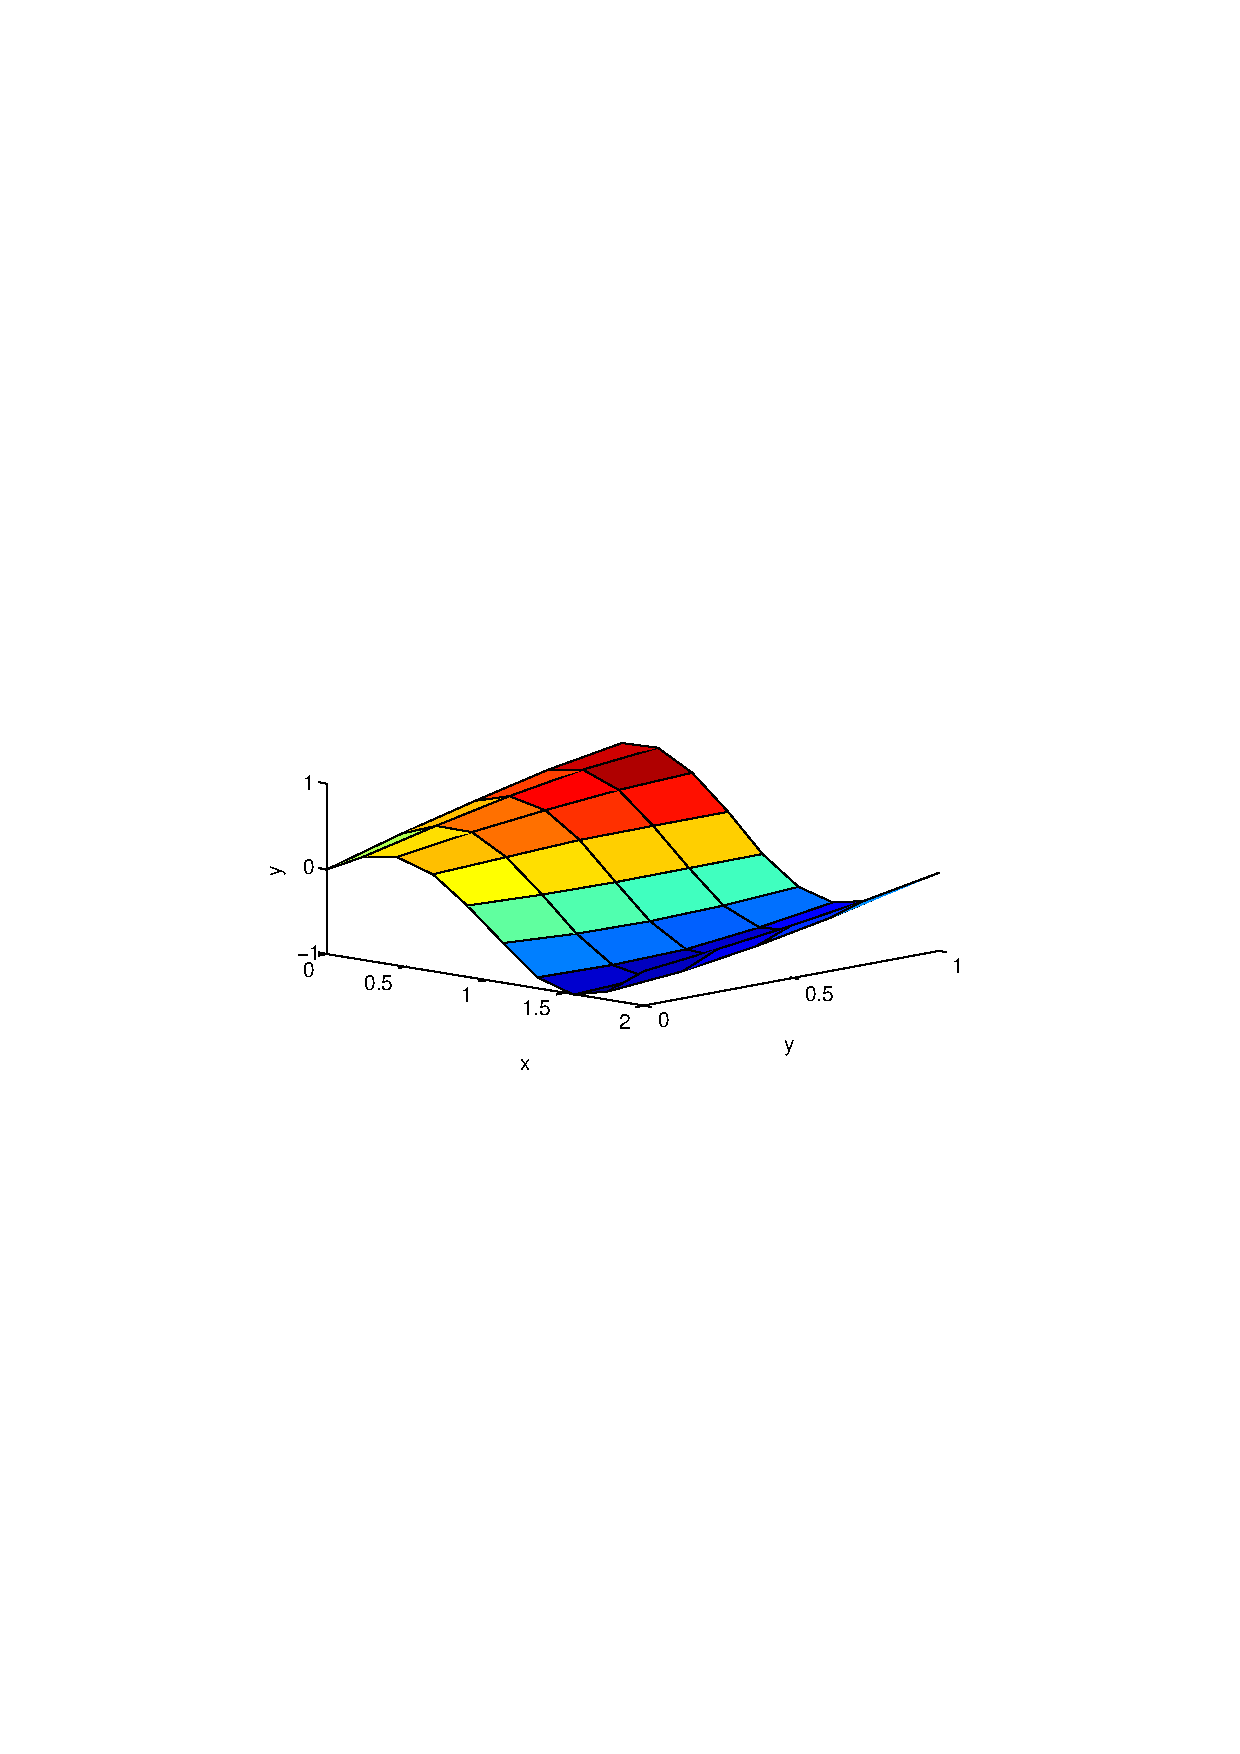
\includegraphics[width=0.45\linewidth, trim=3cm 11cm 3cm 11cm]{figure/X.pdf}
%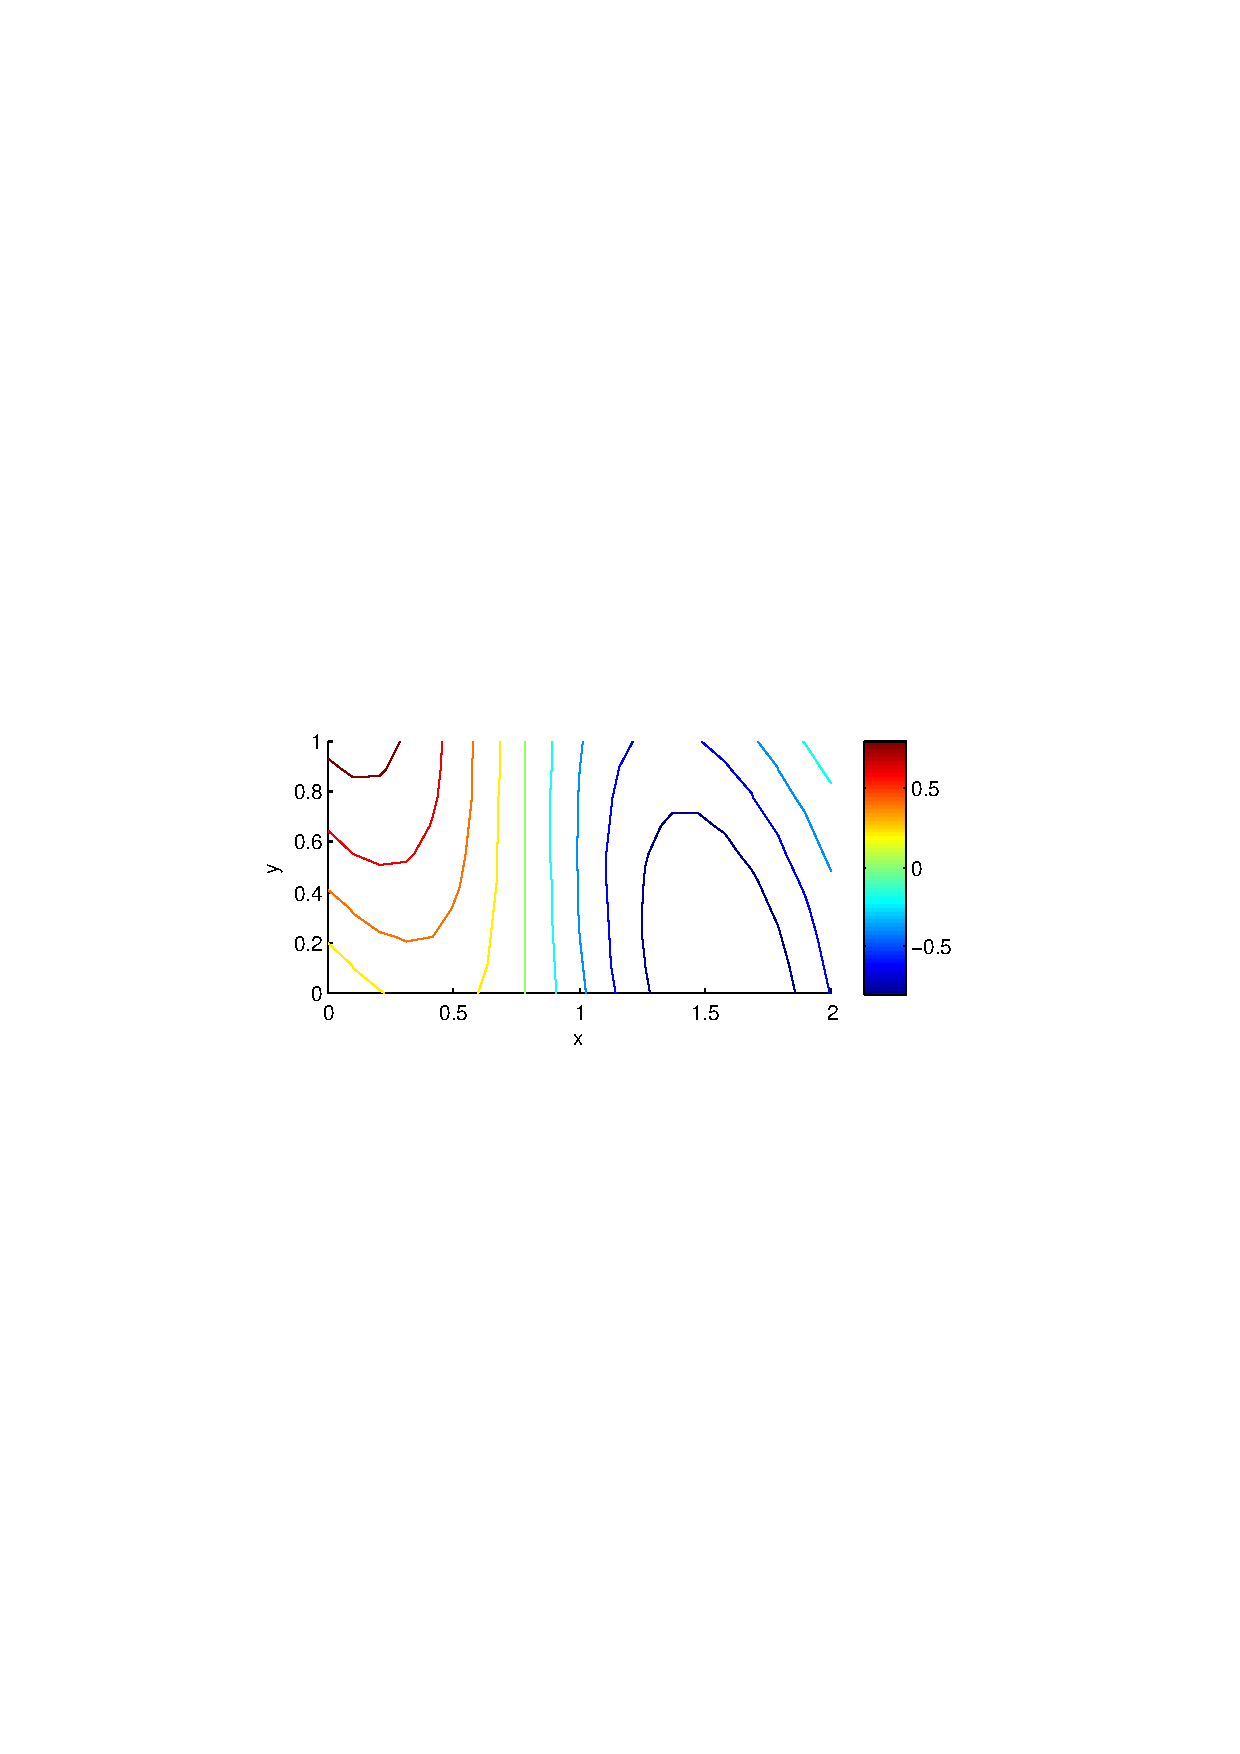
\includegraphics[width=0.45\linewidth, trim=3cm 11cm 3cm 11cm]{figure/Y.pdf}
%\caption{Surface and contour plots showing the two dimensional function $z(x,y)=\sin(x+y)\cos(2x)$.}
%\end{figure}




%\section{Source code listing}
%\begin{minted}[frame=single]{python}
%def em_algorithm(word_counts,
%                 probs,
%                 word_probs,
%                 word_possibilities,
%                 convergence_threshold,
%                 langs):
%    convergence_diff = convergence_threshold
%    expected_counts = dict()
%    expected_fun_counts = dict()
%    
%\end{minted}
